\subsection{Exercise 1}

\subsubsection{Brief description}


In this exercise, I've uploaded the following to retrocomputing:
\begin{itemize}
    \item \textbf{Metal Slug Series - Main games}: about 10 games from the Metal Slug series, which are the main games in the series.
    \item \textbf{Flight Simulator Series}: about 10 games
    \item \textbf{Street Fighter Series}: about 8 games
    \item \textbf{Dragon Ball Games}: about 15 games
    \item About 5 console games
    \item About 5 company
    \item For each videogame, which is a software, I've added information with the relationship \textit{producedBy} to the company that produced it
    \item For each console the producer (I also add the produced for already existing consoles)
    \item I've added my city and nearby cities (about 30)
\end{itemize}



\subsubsection{Improvements to the ontology}
I suggest to add the following updtates to the ontology:
\begin{itemize}
    \item \textbf{First Person Shooter}: I suggest to add the class \textit{First Person Shooter} to the ontology as subclass of \textit{Videogame}
    \item \textbf{Fighting Game}: I suggest to add the class \textit{Fighting Game} to the ontology as subclass of \textit{Videogame}
    \item \textbf{Action Game}: I suggest to add the class \textit{Action Game} to the ontology as subclass of \textit{Videogame}
    \item \textbf{Sandnox Game}: I suggest to add the class \textit{Sandbox Game} to the ontology as subclass of \textit{Videogame}
    \item For software the relationship developedBy involves software and Person. However, in many cases (e.g. videogames) the software is developed by an Organization. I suggest to add this update to the ontology as well.
    \item I would add a relationship \textit{runOn} between the class \textit{Software} and the class \textbf{Operating System} to indicate the operating system on which the software runs.
    \item I'dd add also \textit{executedOn} between the class \textit{Videogame} and the class \textbf{Console} to indicate the console on which the videogame runs.
    \item 
\end{itemize}


\subsubsection{Bugs and improvements in the interface}
I was linking together the videogames and the companies that produced them. I clicked on Entity on the object and an execption page appeared. 
Even after restarting my computer and deleting the cache, the problem persists (here's a screenshot of the error) but changing the browser solved the problem.
\begin{figure}[H]
    \centering
    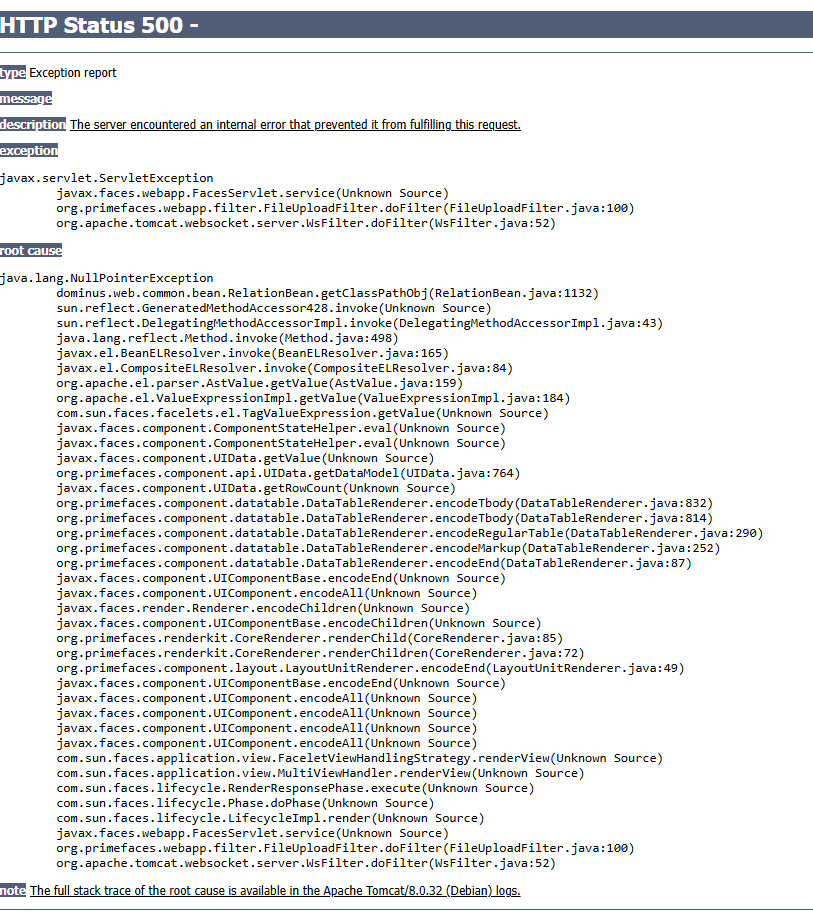
\includegraphics[scale=0.5]{images/exception1.png}
\end{figure}

When I want to add a new relationship, I can't start from the Object but only from the Subject.